\chapter{Marco Teórico}

\section{Introducción}

En este capítulo se sentarán las bases teóricas que soportan y respaldan el trabajar con el algoritmo escogido.

\section{Aplicaciones y aproximaciones en sistemas de posicionamiento indoor}

En cuánto a los sistemas de posicionamiento indoor, diversas documentaciones revisadas señalan la importancia de desarrollar esta tecnología a fin de resolver necesidades ya reconocidas dentro de espacios interiores tales como hospitales, museos, parques, etc. Sin embargo, todos concuerdan en que la tarea no es sencilla y por este motivo se ha intentado abordar este problema de distintas maneras, teniendo cada una sus respectivas ventajas y limitaciones.

La clasificación de estos métodos pasa por si es que en ellos se utilizan propiedades físicas o bien, reconocimiento de imágenes. De este modo, un posible ordenamiento es el que sigue:

\begin{itemize}
    \item{Análisis de escena}
    \item {Detección de proximidad}
    \item{Triangulación}
\end{itemize}

\subsection{Análisis de Escena}
El algoritmo de análisis de escena se refiere al tipo de algoritmo que primero recolecta características de una sala, habitación o espacio y luego estima la posición del objetivo según coincidan los elementos del espacio.

Este algoritmo tiene la ventaja de entregar precisión, a la vez de no requerir la localización de los AP WiFi, y por ende, juega un rol sumamente relevante dentro del algoritmo de posicionamiento indoor. Sin embargo, las desventajas de estos radica en que, computacionalmente hablando, son altamente costosos y que en realidad, no están orientados a entregar posición, sino a reconocer patrones u objetivos, lo que lleva a no conocer coordenadas y geolocalización.

\subsection{Detección de proximidad}\label{Detección de Proximidad}
Este algoritmo es relativamente simple, pero no preciso. Es, en general, utilizado para apoyar el posicionamiento outdoor, ya que este ayuda a estimar la posición de un objetivo utilizando la relación de proximidad entre un objetivo y los Puntos de Acceso cercanos. Cuando el dispositivo móvil objetivo recibe diferentes señales de los distintos AP, permite asociar la intensidad de señal más fuerte a una ubicación particular. 

La precisión de este algoritmo viene dada por la distribución de densidad y el rango de señal de los AP, de modo que si utilizamos antenas adicionales, podemos mejorar la confiabilidad de los resultados, no obstante, esto podría encarecer la implementación.

\subsection{Triangulación}
Este método utiliza propiedades geométricas de triángulos para determinar la ubicación. Tiene dos derivaciones, angulación y lateración. De la primera, se desprende la  técnica de angulación que se basa en la fase de la señal (AoA), mientras que de la segunda, aquellas basadas en la medida de la propagación por tiempo (ToA, TDOA y RTOF) y en los niveles de intensidad de señal recibida (RSSI). 


\begin{figure}[h!]
    \centering
    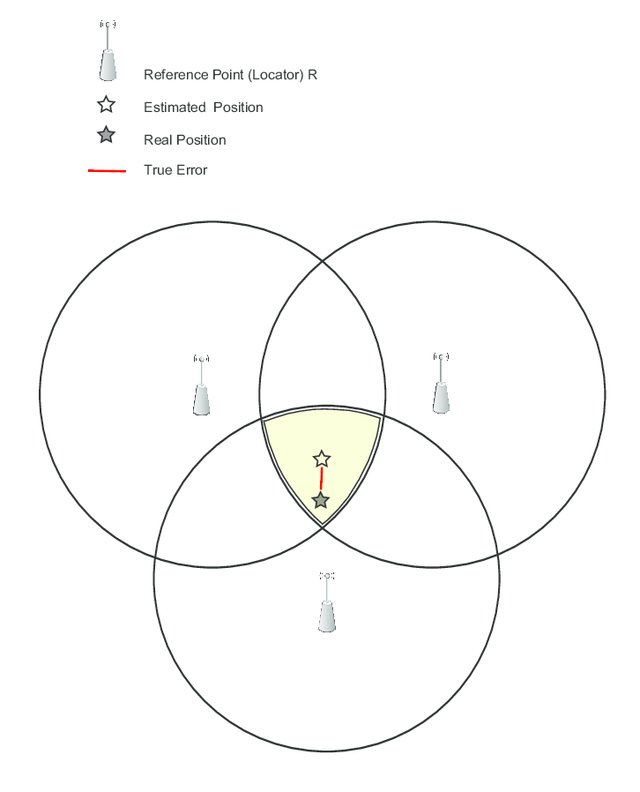
\includegraphics[scale=1]{./images/trilat}
    \caption{Algoritmo de Triangulación}
    \label{fig:Triangulación}
\end{figure}

\subsubsection{\textbf{Angulación}}
    \begin{enumerate}
        \item {\textbf{\ac{AoA}}: es una técnica que determina el ángulo de llegada de la señal, respecto de la ubicación conocida de estaciones base a través de envío de múltiples mensajes desde el Dispositivo móvil hacia el AP. Dado que la precisión de la medición del ángulo de llegada es la que permite estimar la posición, se tiene que estas deben ser altamente direccionales o bien, tratarse de un arreglo de antenas, lo que encarece el costo de sistemas que implementen este tipo de solución. Además, se tiene que esta técnica ve alteradas sus mediciones debido a efectos de la propagación multicamino de la señal cuando se trata de dispositivos que no se hallan en \ac{NLOS}.
        
        \begin{figure}[h!]
            \centering
            \begin{subfigure}[b]{0.3\textwidth}
               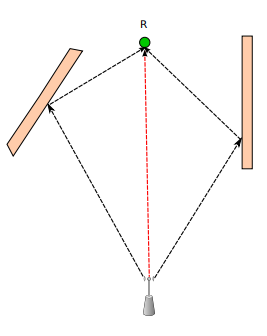
\includegraphics[width=\textwidth]{./images/los}
                \caption{Señal enviada en \ac{LOS}}
                \label{fig:LOS}
            \end{subfigure}
            \begin{subfigure}[b]{0.315\textwidth}
             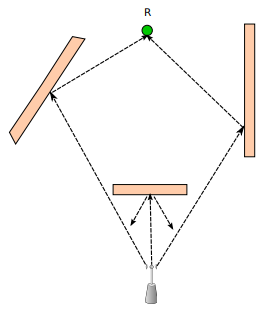
\includegraphics[width=\textwidth]{./images/nlos}
                \caption{Señal enviada en \ac{NLOS}}
                \label{fig:NLOS}
            \end{subfigure}
        \end{figure}
        
%%%%%%%%%%%%%%%%%%%%%%%%%%%%%%%%%%%%%%%%%%%%%%%%%%%%%%%%%%
                \clearpage 
%%%%%%%%%%%%%%%%%%%%%%%%%%%%%%%%%%%%%%%%%%%%%%%%%%%%%%%%%%

        
        Por esta razón, el sistema, aunque preciso en espacios exteriores, no es del todo idóneo para espacios interiores, ya que las reflexiones que se producen en paredes y otros objetos que cambian significativamente la dirección o ángulo de llegada de la señal y por tanto, degradan la precisión de la estimación de posición.
        
        \begin{figure}[h!]
            \centering
            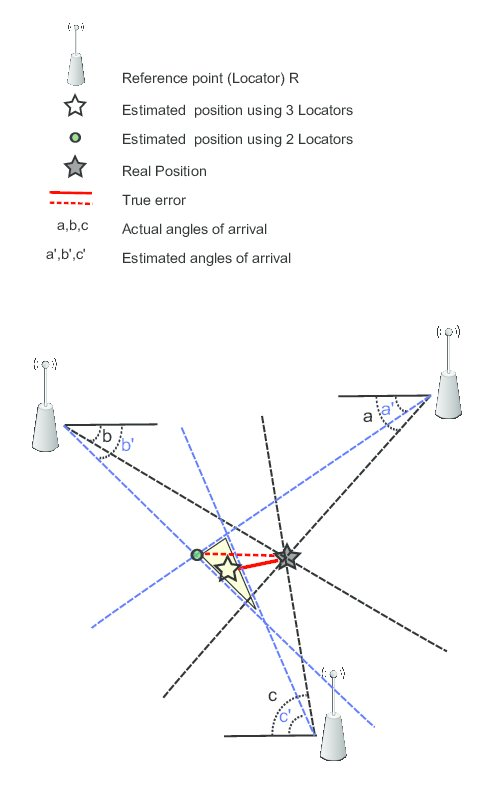
\includegraphics[scale=1.2]{./images/aoa}
            \caption{Técnica de Ángulo de Llegada (AoA)}
            \label{fig:AoA}
        \end{figure}
        }
    \end{enumerate}

%%%%%%%%%%%%%%%%%%%%%%%%%%%%%%%%%%%%%%%%%%%%%%%%%%%%%%%%%%
                \clearpage 
%%%%%%%%%%%%%%%%%%%%%%%%%%%%%%%%%%%%%%%%%%%%%%%%%%%%%%%%%%

\subsubsection{\textbf{Lateración}}

\begin{itemize}
    \item{\textbf{Técnicas basadas en la propagación por tiempo}
    
    \begin{enumerate}
        \item {\textbf{\ac{ToA}}: \label{ToA} El tiempo de llegada aparece como el tiempo de viaje del transmisor hasta el receptor y permite, si es que se le multiplica por la velocidad de la luz, obtener la distancia que separa ambos dispositivos. Para medir el tiempo de llegada en el aire, este método requiere sincronización previa de los dispositivos, que para hacer posicionamiento en el espacio, requiere de al menos 4 transmisores.
        
         \begin{figure}[h!]
            \centering
            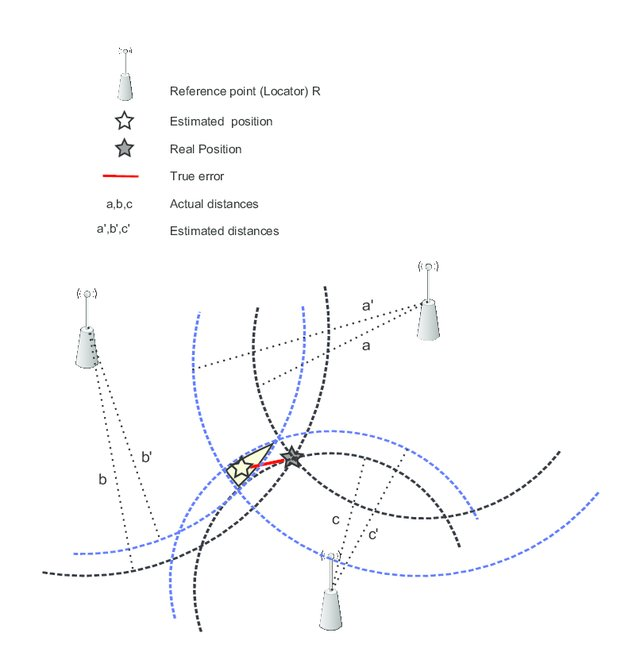
\includegraphics[scale=1]{./images/toa}
            \caption{Técnica de Tiempo de Llegada (ToA)}
            \label{fig:ToA}
        \end{figure}
            
        En ésta técnica, dado que los errores de estimación de distancia se derivan de mediciones de tiempo de salida y llegada del mensaje, se debe procurar que los tiempos sean bien medidos, esto es, que todos los dispositivos transmisor y receptor estén sincronizados en el mismo tiempo. La correcta implementación de un sistema de medición basado en ToA permite filtrar los efectos de la multitrayectoria.\\}
        
        \item {\textbf{\ac{TDoA}}: Esta técnica, acorde a lo mencionado en \cite{17}, cosiste en medir la diferencia de tiempo de llegada de la señal que se envia desde un objeto y que es recibida por otros tres dispositivos.\\
        
        Con TDoA, se puede iniciar la transmisión de la señal en un tiempo desconocido en tanto sea conocido por los otros nodos receptores. Lo único que se requiere para que esto funcione, es que entre los receptores, exista una sincronización de tiempo. Esta técnica, también conocida como Multilateración tiene como obstáculo el hecho de requerir una cantidad significativa de ancho de banda, así como también, el alto costo del equipamiento utilizado para aplicarlo.\\
        
        Y es que la banda usada para la implementación de esta tecnología es la \ac{UWB}, definido por la \ac{FCC} como la porción del espectro electromagnético con frecuencias que van desde los 3.1 hasta los 10.6 GHz.
        
            \begin{figure}[h!]
                \centering
                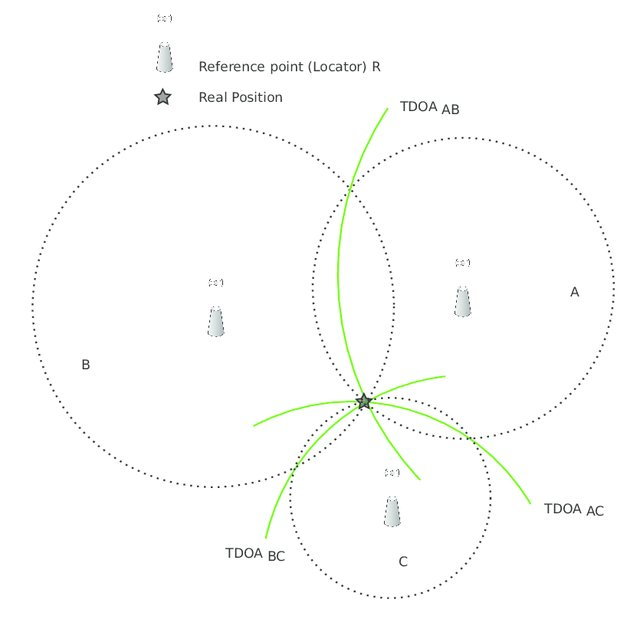
\includegraphics[scale=1]{./images/tdoa}
                \caption{Técnica de Diferencia de Tiempo de Llegada (TDoA)}
                \label{fig:TDoA}
            \end{figure}
        
        }
        \newpage 
        \item {\textbf{\ac{RToF}}: en este método basado en \ref{ToA} que consiste en el tiempo total que toma la conexión entre los dos dispositivos que participan en la comunicación. A diferencia de \ref{fig:TDoA}, acá se considera el tiempo de ida y regreso de la señal, no sólo el tiempo que tarda desde el transmisor hasta el receptor. Este método de medida no requiere ninguna sincronización entre los dispositivos, de modo que se puede implementar necesitan únicamente enviar el resultado de la medición del \ac{RTT} para hacer el cálculo bajo la siguiente fórmula:\\
        
        \begin{equation}
            d = \dfrac{c\cdot{\left(T_{Total} - T_{proc}\right)}}{2}
        \end{equation}
        
        Donde \textit{d}, representa la distancia entre los dos dispositivos; \textit{c}, la velocidad de la luz; Tproc, el tiempo que le toma a la estación realizar el calculo. Siendo este último, un parámetro complejo de obtener con precisión, ya que depende de la latencia del sistema. Esto se escala como la principal desventaja de este sistema ya que calcular la posición para varios dispositivos se traduce en lidiar con latencias que impidan obtener la posición de dispositivos que se mueven rápidamente.
        
        \begin{figure}[h!]
            \centering
            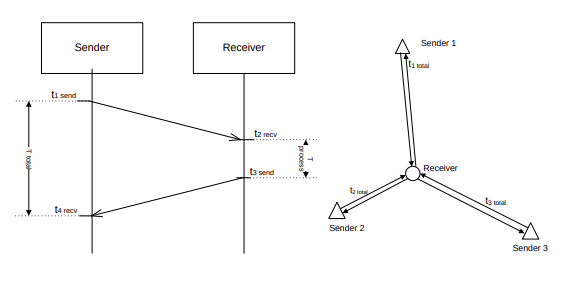
\includegraphics[scale=0.52]{Tesis/images/rtof}
            \caption{Diagrama de medición de distancia usando \ac{RToF}}
            \label{fig:RTOF}
        \end{figure}
        }
    \end{enumerate}
            }

    \item{\textbf{Técnicas basadas en los niveles de intensidad de señal recibida}
    \begin{enumerate}
        \item{\textbf{\ac{RSSI}}: Respecto de esta técnica se tiene que algunos autores la introducen como una técnica propia de algoritmos de Detección de Proximidad (\ref{Detección de Proximidad}}) debido a que los niveles de los indicadores de intensidad de señal recibida, al guardar relación con la distancia, tal y como señalan los modelos de propagación para interiores, establecen que a menor distancia del AP, mayor debe ser la intensidad de señal recibida.\\
        
        Los mismos autores que la clasifican dentro de la sección mencionada, utilizan esta técnica para trazar un sistema de coordenadas basadas en las intensidades recibidas respecto de cada AP, esto les permite mapear la zona en una etapa que llaman offline y ubicar al dispositivo en la etapa posterior, llamada online.\\
            
        En esta etapa, se asigna a través de un sistema de coordenadas, los niveles de intensidad de señal, tal que es posible posicionar el objetivo según los RSS de los AP, como se ve en la imagen.
            
        \begin{figure}[h!]
            \centering
            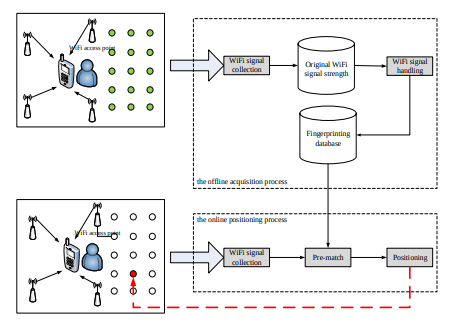
\includegraphics[scale = 0.6]{./images/rssi}
            \caption{Idea de algoritmo basado en RSSI}
            \label{fig:RSSI}
        \end{figure}
        
        \item{Algoritmos de posicionamiento para método por características de posición}\\
        
            \begin{enumerate}
                \item {\textbf{Método Probabilístico}: En este método, se considera el estimar la posición del ibjetivo, como un problema de clasificación, ya que desde un vector de RSS capturadas desde los APs, se puede estimar la probabilidad de que un valor \textit{S}, pertenezca a un AP particular, y por ende, a un punto de coordenadas aproximado. \\
                
                Se puede hacer el cálculo de la posición a través de modelos de inferencia y asociarlo también a un tipo de Cadenas de Markov, así como también, apoyar el cálculo introduciendo medidas de dispersión tales como la desviación estándar y la varianza, o de una medida de tendencia central como es la media.\\
                }
                
%%%%%%%%%%%%%%%%%%%%%%%%%%%%%%%%%%%%%%%%%%%%%%%%%%%%%%%%%%
                \clearpage 
%%%%%%%%%%%%%%%%%%%%%%%%%%%%%%%%%%%%%%%%%%%%%%%%%%%%%%%%%%
                
                \item{\textbf{Método \ac{SVM}}: \label{SVM} En la literatura consultada \cite{7} los autores señalan a esta técnica como \textit{''Una nueva u prometedora técnica para clasificación de datos y Machine Learning.''}, que ha sido usada con resultados satisfactorios en el mapeo de intensidad de señales inalámbricas.\\
                
                Su implementación consiste igualmente en dos fases; una de entrenamiento, que es aquella en que los sets con los datos de  intensidad de señal de los AP son ingresados, y con los cuales se buscará diseñar un hiperplano que clasifique los vectores en dos clases, procurando maximizar la distancia entre estos.\\
                
                \begin{figure}[h!]
                    \centering
                    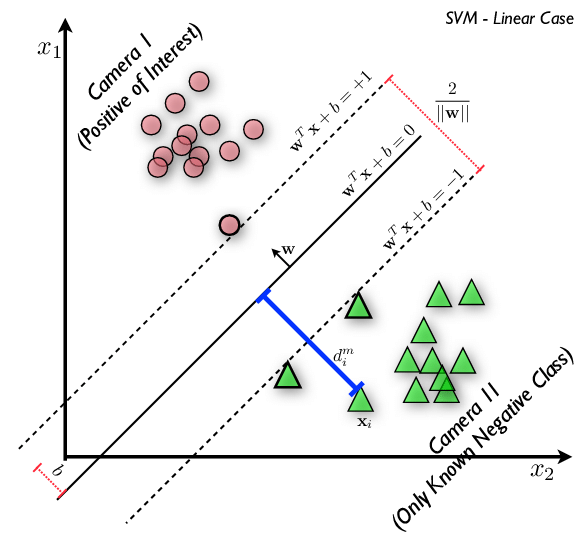
\includegraphics[scale=0.4]{./images/svm}
                    \caption{Distintos hiperplanos para el mismo set de datos.}
                    \label{fig:SVM}
                \end{figure}
                
                Sin embargo, dado que en un espacio indoor, la cantidad de AP es , por lo general, superior a 2, la posibilidad de que en un set de datos podamos diferenciar entre un AP u otro mediante el procedimiento de encontrar el hiperplano que separa maximizando la distancia entre los valores, es nula, e implementar un algoritmo recursivo que vaya evaluando para cada AP, el hiperplano que clasifica la medición del objetivo en alguno de ellos, es costosa computacionalmente además de compleja.\\
                }
%%%%%%%%%%%%%%%%%%%%%%%%%%%%%%%%%%%%%%%%%%%%%%%%%%%%%%%%%%
                \clearpage 
%%%%%%%%%%%%%%%%%%%%%%%%%%%%%%%%%%%%%%%%%%%%%%%%%%%%%%%%%%

                \item {\textbf{Método \ac{KNN}}: El método de vecinos más cercano es uno de los métodos de clasificación más simple dentro de la librería de Machine Learning ya que consiste, en una clasificación por similitud respecto de otros puntos en un dataset de entrenamiento. \\

                El objetivo de este método es el de agrupar vectores de características, que no son más que representaciones matemáticas para la información. Ha de tenerse en cuenta que el vector de características puede requerir un pre procesamiento si es que estas no son necesariamente numéricas, ya que de este modo se podrá agrupar los datos como si se tratara de un vector de $R^{N}$.\\

                Ahora, a diferencia de otros métodos de clasificación, como es el caso de \ref{SVM}, en KNN la fase de entrenamiento no existe, de manera que sólo se trata de una fase. En cambio, se tiene que cualquier caso por abstraer o generalizar la información que allí está, es un hecho en la etapa de clasificación.\\

                Esto significa que se puede trabajar inmediatamente sobre los datos, en tanto estos, tal y como se mencionó previamente, no requieran un pre procesamiento. Dado que lo que hace este método es agrupar valores, el resultado óptimo será cuando exista un reducido número de  data-sets y estos no tengan valores no numéricos.\\

                Así, se tiene que los datos que se clasificarán pueden también ser representados como una matriz de M x N  datos, de donde ; M, es el número de datos; y N, son las características de los datos. Dicho esto, el proceso de agrupamiento de los datos se hace según las siguientes consideraciones:\\

                \begin{itemize}
                    \item {Se calcularán las distancias entre los valores a clasificar, y aquellos contenidos en el data-set. En el cálculo de la distancia suele usarse la distancia euclidiana, que es básicamente, la magnitud del vector que se obtiene al restar un punto de muestra del data-set de entrenamiento, con el punto a clasificar
    
                    \begin{equation}
                        E(x,y) = \sqrt{\sum_{i=0}^{n}({x_{i}-y_{i}})^{2}} \ \ 
                    \end{equation}
                    }

                    \item{Se escogerá un valor \textit{K}, que por lo general, no es ni múltiplo de la cantidad de clases, ni par, y que representa la cantidad de valores \textit{K} con las distancias más bajas. Este puede ser escogido arbitrariamente o bien, en caso que sea necesario, obtenido por validación cruzada. \footnote{La validación cruzada o cross-validation es una técnica utilizada para evaluar los resultados de un análisis estadístico y garantizar que son independientes de la partición entre datos de entrenamiento y prueba.}\\}
                    
                    \item{Finalmente, se agruparán los datos a una clase, a través de la comparación de las distancias obtenidas. Si este, posee la mayoría de los  \textit{K} de puntos cuya distancia los asocia a una clase A, entonces este será clasificado en dicha clase. Si por el contrario, el número de puntos cuya distancia se acerca a los datos objetivo no son mayoría, entonces este pertenecerá a B.\\
                    
                    \begin{figure}[h!]
                        \centering
                        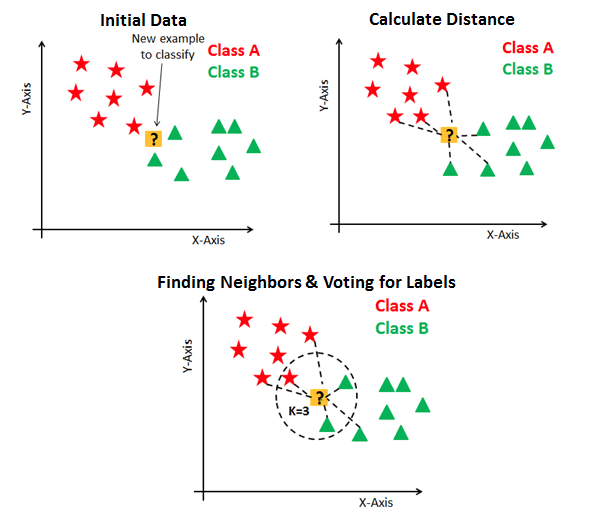
\includegraphics[scale=0.65]{./images/knn}
                        \caption{Representación gráfica del funcionamiento de KNN según el valor de K}
                        \label{fig:KNN}
                    \end{figure}
                    }
            \end{itemize}}
            
            \newpage
            
            \item{\textbf{Método \ac{RNA}}: Este método se vale de una neurona artificial llamada \textbf{perceptrón}, algo que fuera desarrollado entre los años 1950s y 1960s por el científico Frank Rosenblatt, inspirado por el trabajo de Warren McCulloch y Walter Pitts <<A Logical Calculus of the Ideas Immanent in Nervous Activity>> \cite{19} donde señalan la posibilidad de rescatar la idea de un sistema complejo de redes y conexiones, de impulsos y señales, como es nuestro sistema nervioso, y extrapolarlo a uno computarizado, donde en lugar de estímulos, se tuvieran señales.\\
            
             Se mencionó que uno de los objetivos del trabajo de McCulloch fue el de introducir la noción de neurona artificial, por esto es que el perceptrón le debe su estructura, presentada a continuación:
             
            \begin{figure}[h!]
                \centering
                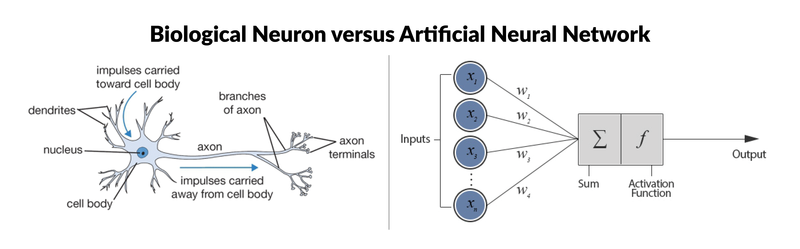
\includegraphics[scale=0.5]{Tesis/images/nn}
                \caption{Comparación por similitud de una neurona con un perceptrón}
                \label{fig:NN}
            \end{figure}
            
            En el cerebro humano, existen distintos tipos de neuronas las cuales están destinadas para tareas específicas, por esta razón, puede darse que una neurona reciba señales de temperatura, presión, luz, entre otras, antes de transmitir un impulso. Este último viene en algunos casos a ser la suma ponderada de los distintos estímulos nerviosos que provienen de las otras terminaciones sinápticas, tal que es en el soma donde se evalúa si esta excede el potencial de acción o no. Si lo hace, la señal será enviada a través del soma y las terminaciones sinápticas hasta un órgano diana u otra neurona, pudiendo ser esta señal inhibitoria, excitadora o moduladora.\\
            
            \begin{figure}
                \centering
                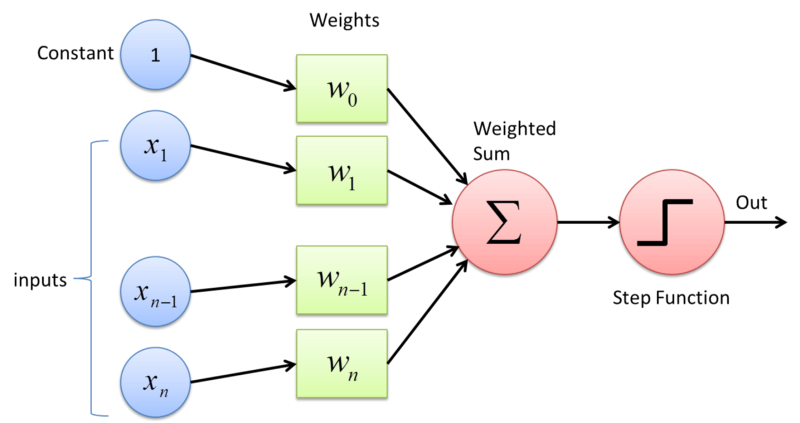
\includegraphics[scale=0.35]{Tesis/images/perceptron}
                \caption{Representación de un Perceptrón}
                \label{fig:Perceptron}
            \end{figure}
            
            Tal como se puede ver en \ref{fig:Perceptron}, se tiene que están las conexiones de la capa de entrada, representadas por impulsos o señales de entrada \textbf{$x_j$}, que luego se multiplican por los pesos \textit{$w_j$} y pasan a evaluarse en la función de activación.\\
            
            Las neuronas son representadas como unidades individuales de procesamiento, que al agruparse forman una red neuronal cuya función de activación, y luego, las capas se resumen en tres:\\
            
            \begin{itemize}
                \item {\textbf{Capa de entrada}: las unidades que componen esta capa son los campos de entrada, por donde ingresan los primeros estímulos}
                
                \item{\textbf{Conexiones ponderadas}: Las operaciones que se realizan en las capas, se logran a través de las fuerzas de conexión variables, o ponderaciones, que resultan del producto entre los pesos \textbf{$w_j$}, que representan la fuerza que tiene un nodo en particular, y los estímulos \textbf{$x_j$}. Los datos de entrada se presentan en la primera capa y estos se propagan a través de las capas ocultas, en forma de \textit{función de propagación},tal cual hiciera el impulso eléctrico en las neuronas, hasta llegar a la capa de salida que es donde el dato de salida, nos permitirá tomar decisiones o evaluar resultados.}
                
                \item{\textbf{Capas Ocultas}:  Son aquellas unidades de procesamiento que transforman el impulso de entrada en otro diferente pero que no son realmente ni una entrada ni una salida.}
                
                \item{\textbf{Función de activación}: Es quizás la característica principal o definitoria de las neuronas, la que mejor define el comportamiento de la misma. Se usan diferentes tipos de funciones, desde simples funciones simples de umbral a funciones no lineales. Se encarga de calcular el nivel o estado de activación de la neurona en función de la entrada total.\\
                
                La función de activación, en este caso Sigmoide, corresponde una función continua no lineal cuyo rango va entre 0 y 1 que puede ser representada gráficamente a través de \ref{fig:sigmoid} y matemáticamente a través de \ref{sigmoid_eq}:\\
            
                \begin{figure}[h!]
                    \centering
                    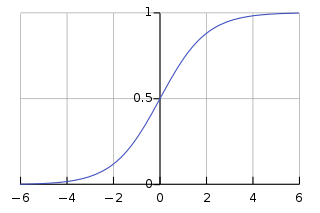
\includegraphics[scale=0.6]{./images/sigmoid}
                    \caption{Función Continua no lineal Sigmoide}
                    \label{fig:sigmoid}
                \end{figure}
            
                \begin{equation}
                    S(u_j) = \dfrac{1}{1+e^{-u_j}}
                    \label{sigmoid_eq}
                \end{equation}
                }       
                
                \item{\textbf{Capa de salida}: Compuesta por una o varias unidades que representan los campos de salida y que entregan el resultado que finalmente es modelado por la siguiente expresión:
                
                \begin{equation}
                    O_j  = S({w_j}{x_j} + {w_0})
                    \label{prob_pred}
                \end{equation}
                
                Donde $w_0$, es el  Bias, una constante que ayuda al modelo de una manera que puede ajustarse mejor a los datos dados y $O_j$, el resultado particular de la evaluación de un dato en la función Sigmoide.\\
                }
            \end{itemize}
            
            Al igual que hace el cerebro por acción de las neuronas, una red es capaz de aprender examinando los registros individuales, generando una predicción para cada uno de estos y ajustando, a través de los pesos, las ponderaciones en caso que el resultado no haya sido el óptimo. Este proceso es iterativo y puede tener lugar cientos de veces antes que la red sea capaz de mejorar sus predicciones antes de alcanzar resultados que satisfagan los criterios de parada.\\
            
            En un comienzo, las ponderaciones son aleatorias, y las respuestas suelen ser muy dispares, sin embargo, y conforme va avanzando el entrenamiento, esta va mejorando, haciéndose más precisa en predecir o replicar a partir de los resultados conocidos.\\
            
            Un aspecto importante, es que a la propagación de las respuestas desde las capas de entrada hacia la capa de salida, se le llama \textit{forward propagation} o \textit{propagación hacia adelante} y cuyo objetivo, así como el del entrenamiento en general es minimizar el costo computacional de la red. Ahora, así como existe la propagación hacia adelante, existe también una hacia atrás llamada \textit{back propagation}, que consiste en reingresar al sistema, la salida resultante de proceso anterior, a fin de optimizar el resultado de los pesos y sesgos. }
            \end{enumerate}
        \end{enumerate}
            }
    \end{itemize}
    